\section{The STR7 Microcontroller Simulator Description}
\label{sec:str7_validation_description}

The STR7 microcontroller is a member of the STMicroelectronics 32-bit microcontroller family combining the industry-standard ARM7TDMI 32-bit core with a comprehensive set of peripherals and a flash memory.

\begin{figure}[!h]
	\begin{center}
		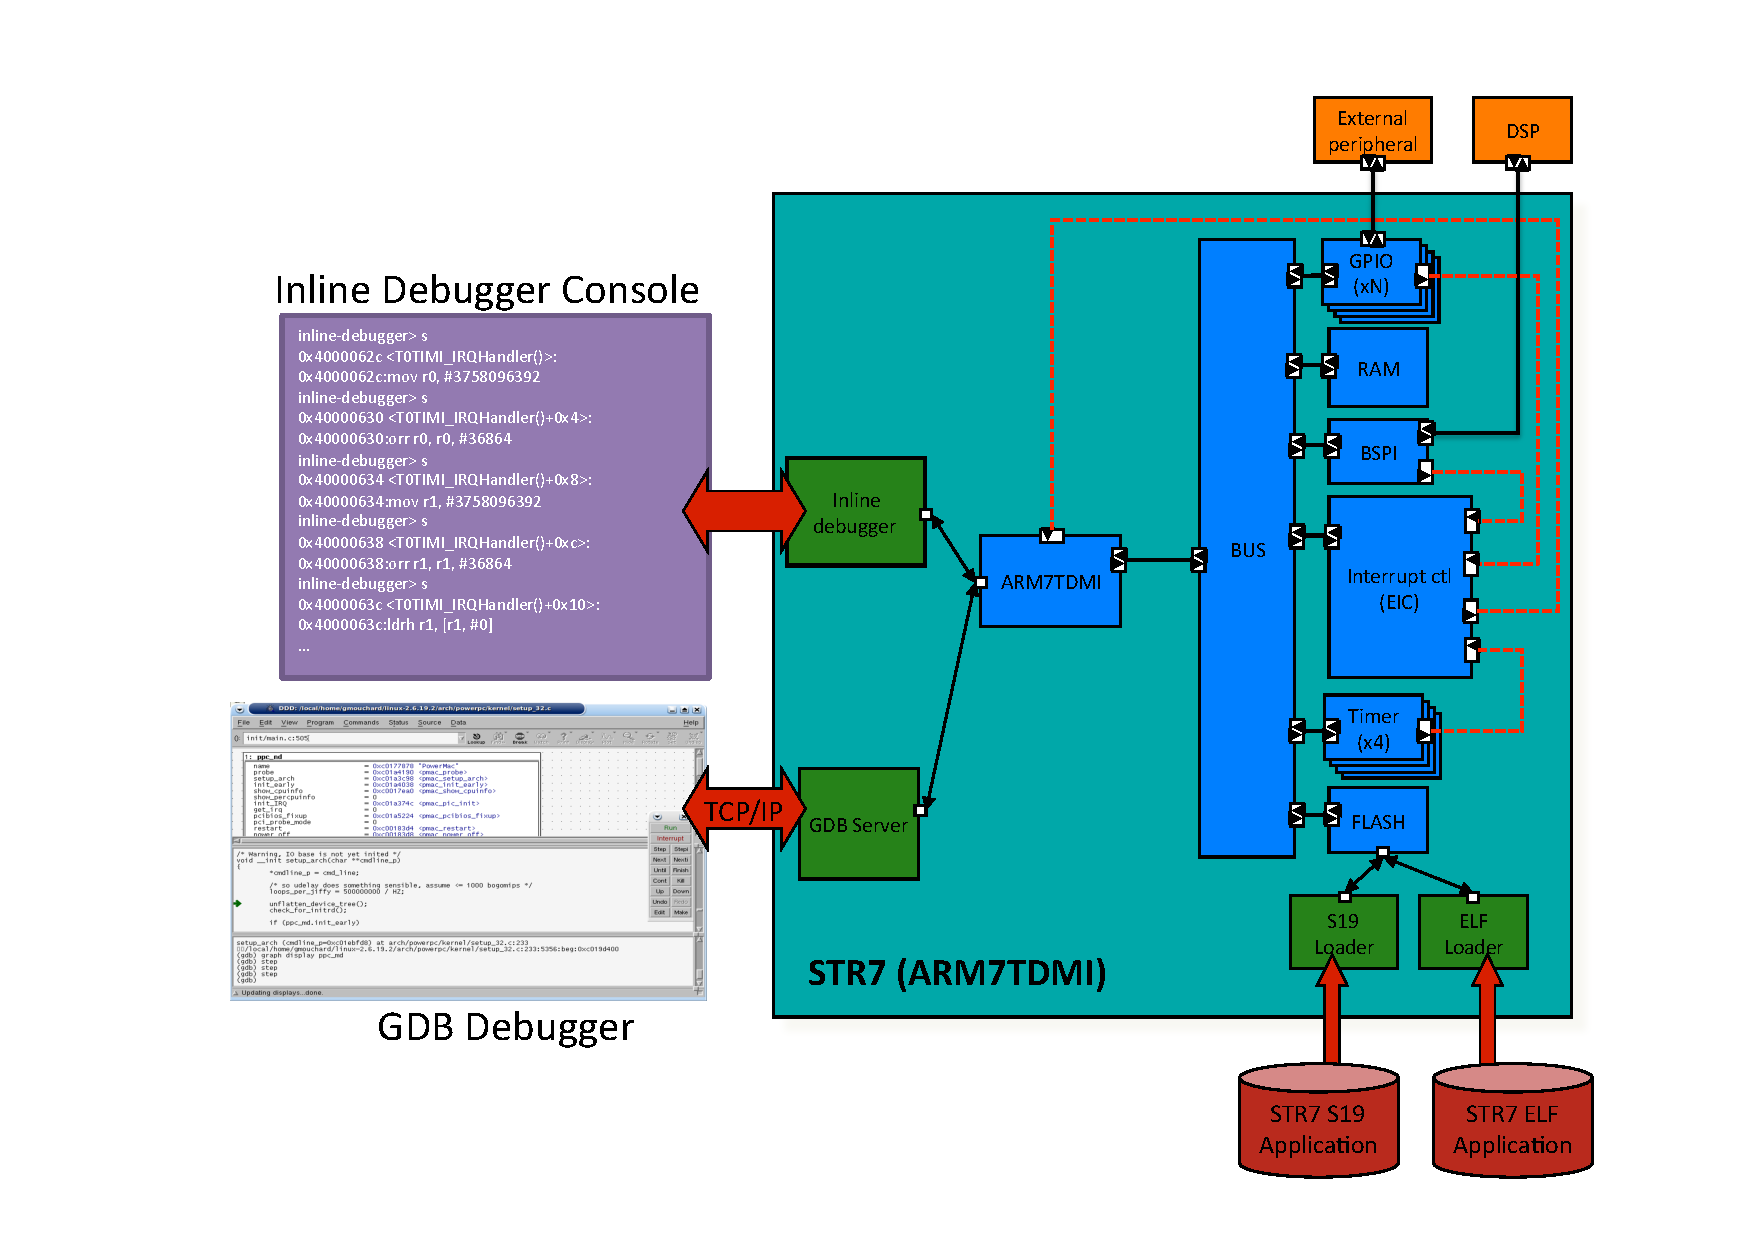
\includegraphics[width=\textwidth]{str7_validation/figures/str7_architecture.pdf}
	\end{center}
	\caption{STR7 schematic architecture.}
	\label{fig:str7_validation_str7_architecture}
\end{figure}

The ARM7TDMI architecture is based on \textit{Reduced Instruction Set Computer} (RISC) principles.
It uses a three-stage pipeline, so instructions are executed in three stages:
\begin{itemize}
	\item Fetch: instruction fetched from memory.
	\item Decode: decoding of registers used in instruction.
	\item Execute: register(s) read from register bank, shift and/or ALU operation, write register(s) back to register bank.
\end{itemize}
A total of 32 registers are available.
However, the processor has seven modes of execution, and while executing in a given mode the processor has only access to a subset (concretely sixteen registers) of them.
Additionally, the ARM7TDMI can execute two different instruction sets (ISAs):
\begin{itemize}
	\item Standard ARM ISA: it is composed of 32 bits RISC instructions. This is the main ISA of the ARM processors series.
	\item Thumb ISA: it is composed of 16 bits RISC instructions. This ISA is used to reduce code footprint, however the number of instructions proposed by this ISA is reduced, so not all kind of operations can done using this ISA.
\end{itemize}
The two ISAs are fully supported by the simulator.

The ARM7TDMI microprocessor is the base of the STR7 family.
The STR7 family extends it with the following peripherals (from the STR71X series):
\begin{itemize}
	\item Memories: Flash and RAM memories, and external memories are supported by the microcontroller.
	\item Nested interrupt controller with support of:
	\begin{itemize}
		\item fast interrupt handling with multiple vectors, 
		\item 32 vectors with 16 IRQ priority levels,
		\item and 2 maskable FIQ sources
	\end{itemize}
	\item Up to 48 I/O ports.
	\item 5 timers, including:
	\begin{itemize}
		\item a 16-bit watchdog
		\item 3 16-bit timers with 2 input captures, 2 output compares, PWM and pulse counter
		\item a 16-bit timer for timebase functions
	\end{itemize}
	\item 10 communication interfaces, including support for BSPI, CAN, and USB among others.
\end{itemize}

Not the complete STR7 system has been implemented under UNISIM, but a subset that includes:
\begin{itemize}
	\item memories,
	\item interrupt controller,
	\item basic GPIO functionality,
	\item timers (with the exception of the 16-bit watchdog),
	\item the BSPI communication interface,
	\item other components where replaced by stubs (ADC, I2C, APB, and PRCCU among others), because they were not used with the applications under test.
\end{itemize}
For the development of the STR7 simulator the following documents were used:
\begin{itemize}
	\item ARM Architecture Reference Manual
	\item ARM7TDMI (Rev 4) Technical Reference Manual
	\item STR71xF microcontroller family Reference Manual (UM0084)
\end{itemize}
Please refer to them if you are looking for more details on the ARM7TDMI processor and the STR7 microcontroller.

Figure~\ref{fig:str7_validation_str7_architecture} shows the schematic architecture of the simulator used for the validation of the STR7 microcontroller.
The simulator itself consist on the following components (the blue boxes on Figure~\ref{fig:str7_validation_str7_architecture}):
\begin{itemize}
	\item \textbf{ARM7TDMI:} this component models the ARM7TDMI processor.
	\item \textbf{System Bus:} this component allows the connection of the ARM7TDMI processor to the main memory.
	\item \textbf{RAM:} this component is the memory of the system. The processor uses it to store temporary information. It can be parametrized as a RAM or SRAM.
	\item \textbf{FLASH:} a flash type memory used by the microcontroller as boot. It is only as a read-only memory in the system under test.
	\item \textbf{GPIOs:} this component is used to perform communication with peripherals external to the microcontroller using the GPIO protocol.
	\item \textbf{BSPI:} this component is used to perform communication with peripherals external to the microcontroller using the SPI protocol.
	\item \textbf{Interrupt Controller:} this component synthesizes and prepares the different system interruptions before handling from the ARM7TDMI processor.
	\item \textbf{Timers:} a series of timers to perform time handling operations.
\end{itemize}

The simulator can be easily extended to use external modules thanks to the GPIO and the BSPI interfaces provided.
Additionally, the simulator provides two services (green boxes on Figure~\ref{fig:str7_validation_str7_architecture}):
\begin{itemize}
	\item \textbf{S19 Loader:} thanks to this service S19 STR7 binaries can be loaded into the FLASH/RAM component.
	\item \textbf{ELF Loader:} thanks to this service ELF STR7 binaries can be loaded into the FLASH/RAM component. The advantage of the ELF loader is that ELF binaries can contain debugging information (like symbols), unlike S19 binaries. This can be helpful when using the debugging tools.
	\item \textbf{GDB Server:} this service enables extended debugging with the help of an external client debugger, as for example: gdb, ddd, eclipse debugger, and others.
	\item \textbf{Inline Debugger:} this service incorporates an extended inline debugger tool to the simulator without the need of a client debugger.
\end{itemize}


